% !TEX program = xelatex
\documentclass[a4paper,14pt,oneside,openany]{memoir}

%%% Задаем поля, отступы и межстрочный интервал %%%

\usepackage[left=30mm, right=15mm, top=20mm, bottom=20mm]{geometry}
\pagestyle{plain}
\parindent=1.25cm
\usepackage{indentfirst}

%%% Задаем языковые параметры и шрифт %%%

\usepackage[english,russian]{babel}
\babelfont[russian]{rm}{Times New Roman}
\babelfont[russian]{tt}{Courier New}

%%% Задаем стиль заголовков и подзаголовков в тексте %%%

\setsecnumdepth{subsection}
\renewcommand*{\chapterheadstart}{}
\renewcommand*{\printchaptername}{}
\renewcommand*{\chapnumfont}{\normalfont\bfseries}
\renewcommand*{\afterchapternum}{\hspace{1em}}
\renewcommand*{\printchaptertitle}{\normalfont\bfseries\centering\MakeUppercase}
\setbeforesecskip{20pt}
\setaftersecskip{20pt}
\setsecheadstyle{\raggedright\normalfont\bfseries}
\setbeforesubsecskip{20pt}
\setaftersubsecskip{20pt}
\setsubsecheadstyle{\raggedright\normalfont\bfseries}

%%% Исправление нумерации секций %%%

\renewcommand{\thesection}{\arabic{section}}
\renewcommand{\thesubsection}{\arabic{subsection}}

%%% Сквозная нумерация рисунков и таблиц %%%

\counterwithout{figure}{chapter}
\counterwithout{table}{chapter}

%%% Выравнивание и переносы %%%

\tolerance 1414
\hbadness 1414
\emergencystretch 1.5em
\clubpenalty=10000
\widowpenalty=10000

%%% Задаем параметры оформления рисунков и таблиц %%%

\usepackage{graphicx}
\usepackage{caption}
\usepackage{subcaption}
\usepackage{float}
\graphicspath{{photo/}}
\captionsetup[figure]{font=small, width=\textwidth, name=Рисунок, justification=centering}
\captiondelim{ --- }
\usepackage[section]{placeins}

%%% Задаем параметры ссылок и гиперссылок %%% 

\usepackage{hyperref}
\hypersetup{
    colorlinks=true,
    linkcolor=red,
    citecolor=red
}

%%% Настраиваем отображение списков %%%

\usepackage{enumitem}
\renewcommand*{\labelitemi}{\normalfont{--}}
\setlist{noitemsep, leftmargin=*}

\begin{document}

% Титульный лист (без номера страницы)
\thispagestyle{empty}

\begin{center}
    МИНИСТЕРСТВО ЦИФРОВОГО РАЗВИТИЯ, СВЯЗИ И МАССОВЫХ \\ КОММУНИКАЦИЙ \\ РОССИЙСКОЙ ФЕДЕРАЦИИ

    \vspace{20pt}

    Федеральное государственное бюджетное образовательное учреждение \\ высшего образования \\
    "Сибирский государственный университет телекоммуникаций и \\ информатики"

    \vspace{20pt}

    Кафедра телекоммуникационных систем и вычислительных средств \\ (ТС и ВС)
\end{center}

\vfill

\begin{center}
    Практическая работа №5 \\
    по дисциплине \\
    \textit{"Web-технологии"}

    \vspace{20pt}

    по теме: \\
    \uppercase{Настройка DNS+DHCP сервера для локальной сети}
\end{center}

\vfill

\noindent Студент: \\
\textit{Группа ИКС-532 \hfill А.С. Лёшин}

\vspace{20pt}

\noindent Преподаватель: \\
\textit{старший преподаватель \hfill А.В. Андреев}

\vfill

\begin{center}
    Новосибирск 2026 г.
\end{center}

\newpage
\setcounter{page}{2}
\OnehalfSpacing*

\section*{Введение}
\addcontentsline{toc}{section}{Введение}

В современных корпоративных сетях важную роль играют службы DNS и DHCP. DNS (Domain Name System) обеспечивает преобразование доменных имен в IP-адреса, а DHCP (Dynamic Host Configuration Protocol) автоматически назначает IP-адреса устройствам в сети. Особый интерес представляет их совместная работа, когда DHCP-сервер может динамически обновлять DNS-записи, что значительно упрощает администрирование сети.

Целью данной работы является настройка DNS-сервера на базе Bind9, DHCP-сервера и организация их совместной работы с возможностью динамического обновления DNS-зон.

\section{Настройка DNS-сервера}

\subsection{Изменение имени хоста}

Первым этапом настройки является изменение имени хоста сервера. На \hyperref[fig:rename1]{рисунке \ref*{fig:rename1}} показан процесс переименования hostname в операционной системе.

\begin{figure}[H]
    \centering
    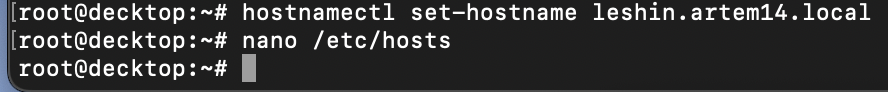
\includegraphics[width=0.8\textwidth]{photo/snimok1.png}
    \caption{Изменение имени хоста}
    \label{fig:rename1}
\end{figure}

Далее необходимо поправить имя сервера в файле \texttt{/etc/hosts}. На \hyperref[fig:rename2]{рисунке \ref*{fig:rename2}} представлено содержимое данного файла после редактирования.

\begin{figure}[H]
    \centering
    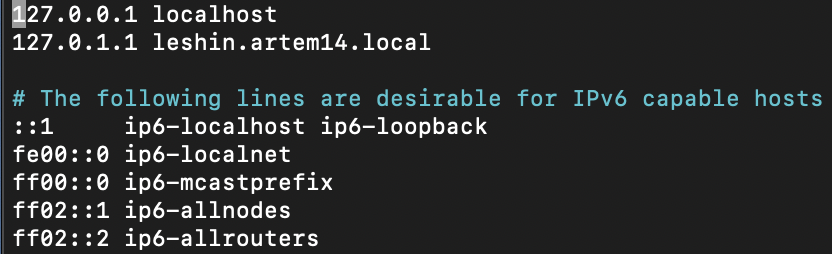
\includegraphics[width=0.6\textwidth]{photo/snimok2.png}
    \caption{Содержимое файла /etc/hosts}
    \label{fig:rename2}
\end{figure}

После сохранения изменений требуется перезагрузка сервера.

\subsection{Установка и настройка Bind9}

Для работы DNS-сервера используется пакет Bind9. На \hyperref[fig:named.conf.option]{рисунке \ref*{fig:named.conf.option}} представлена конфигурация файла \texttt{named.conf.options}, где задаются основные параметры работы сервера.

\begin{figure}[H]
    \centering
    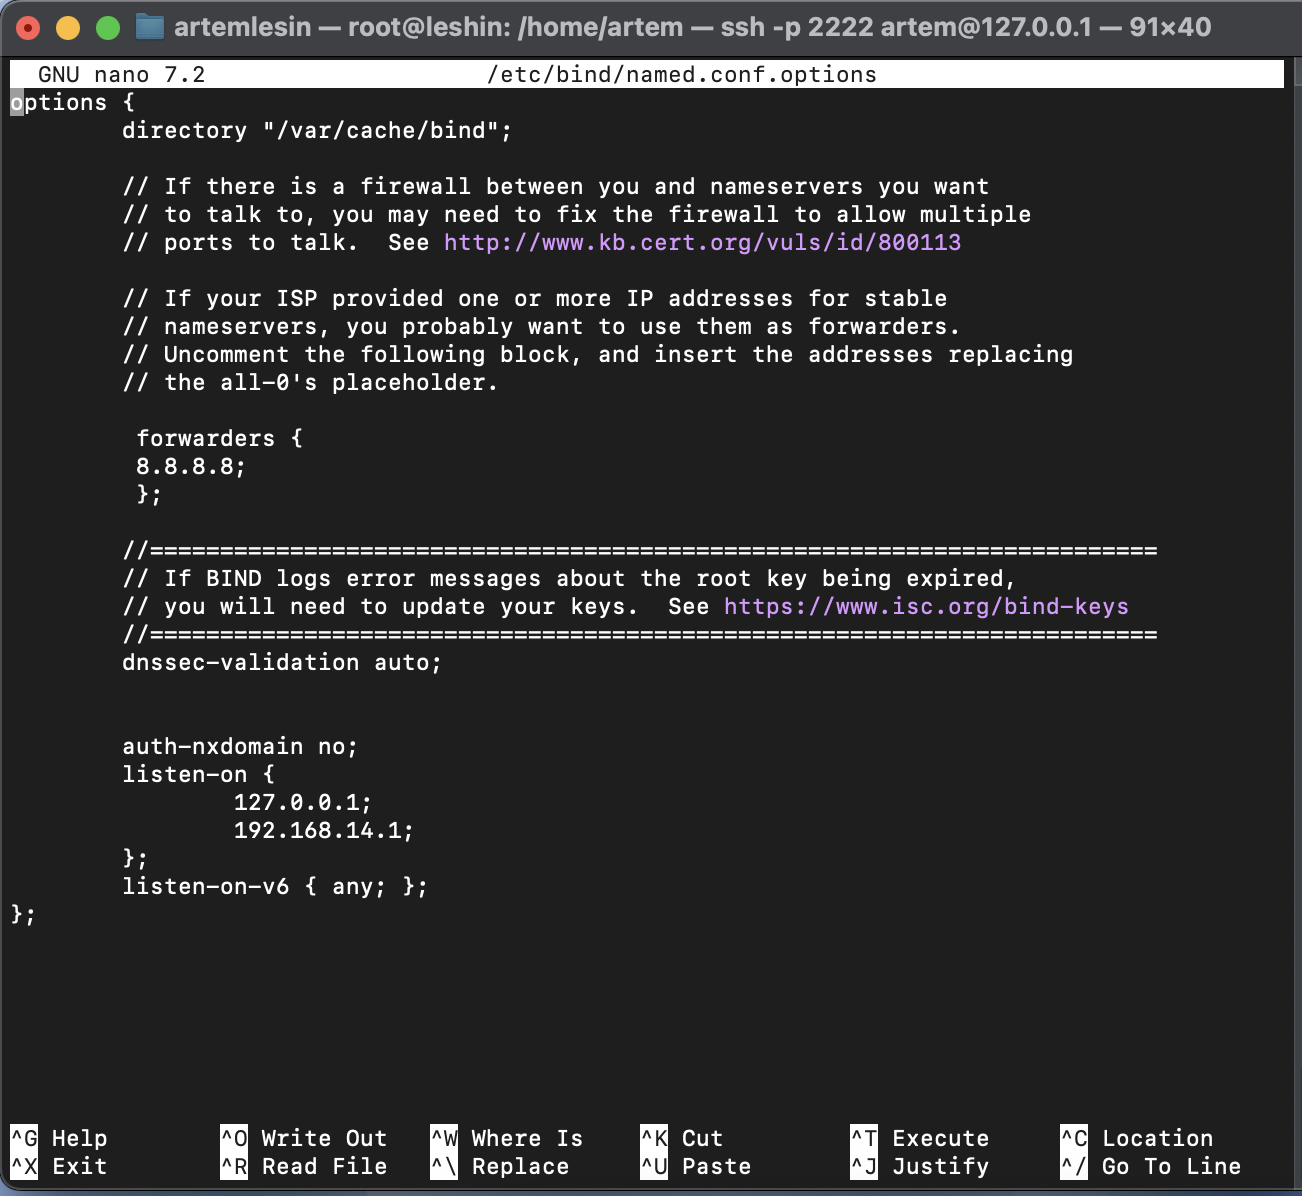
\includegraphics[width=0.6\textwidth]{photo/snimok3.png}
    \caption{Конфигурация файла named.conf.options}
    \label{fig:named.conf.option}
\end{figure}

Далее выполняется редактирование файла \texttt{named.conf.local}, в котором определяются зоны DNS. На \hyperref[fig:named.conf.local]{рисунке \ref*{fig:named.conf.local}} показаны добавленные зоны прямого и обратного просмотра.

\begin{figure}[H]
    \centering
    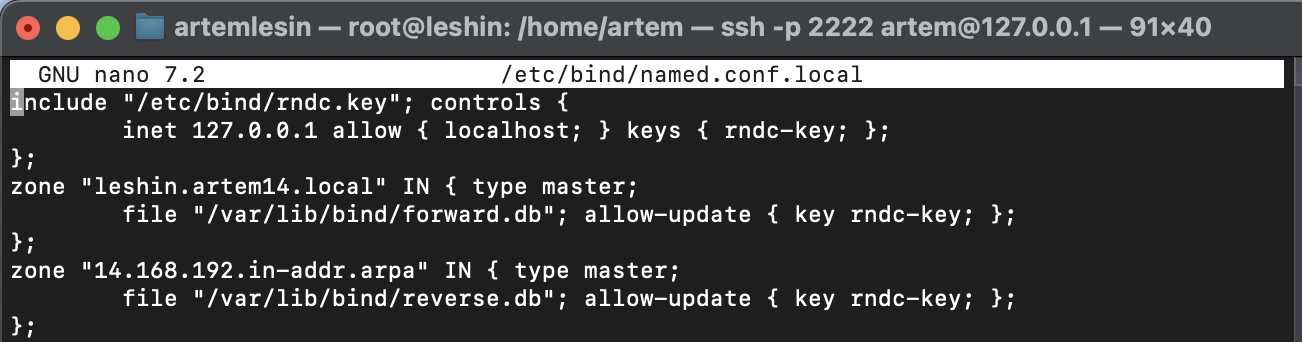
\includegraphics[width=0.8\textwidth]{photo/snimok4.png}
    \caption{Конфигурация файла named.conf.local}
    \label{fig:named.conf.local}
\end{figure}

\subsection{Создание файлов зон}

Для зоны прямого просмотра создается файл \texttt{forward.db}. На \hyperref[fig:forward.db]{рисунке \ref*{fig:forward.db}} представлено его содержимое с записями о соответствии доменных имен IP-адресам.

\begin{figure}[H]
    \centering
    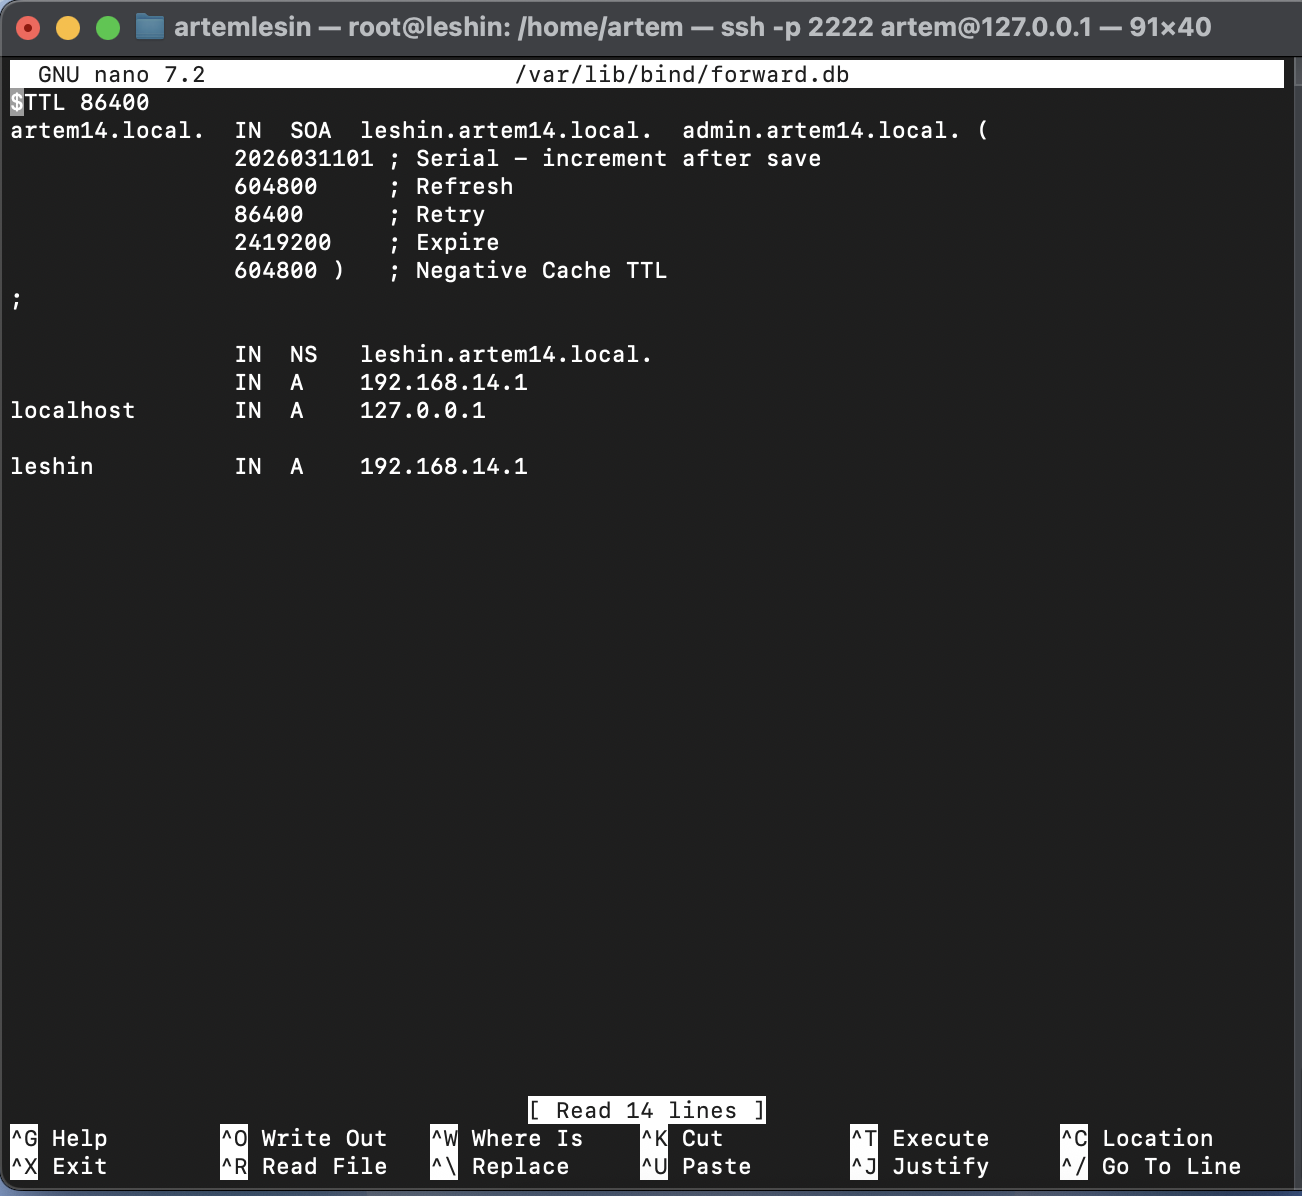
\includegraphics[width=0.6\textwidth]{photo/snimok5.png}
    \caption{Содержимое файла forward.db}
    \label{fig:forward.db}
\end{figure}

Для зоны обратного просмотра создается файл \texttt{reverse.db}, который позволяет выполнять обратное преобразование IP-адресов в доменные имена. На \hyperref[fig:reverse.db]{рисунке \ref*{fig:reverse.db}} представлено его содержимое.

\begin{figure}[H]
    \centering
    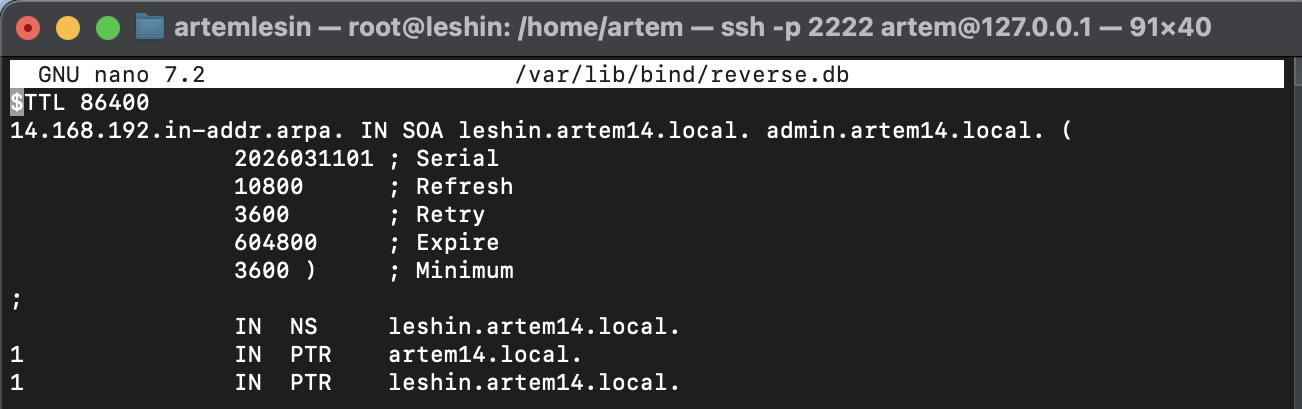
\includegraphics[width=0.8\textwidth]{photo/snimok6.png}
    \caption{Содержимое файла reverse.db}
    \label{fig:reverse.db}
\end{figure}

\subsection{Проверка работоспособности DNS-сервера}

Для проверки работы DNS-сервера необходимо изменить настройки сети, указав в качестве DNS-сервера локальный адрес. На \hyperref[fig:00-installer-config.yaml]{рисунке \ref*{fig:00-installer-config.yaml}} показаны настройки сетевого интерфейса.

\begin{figure}[H]
    \centering
    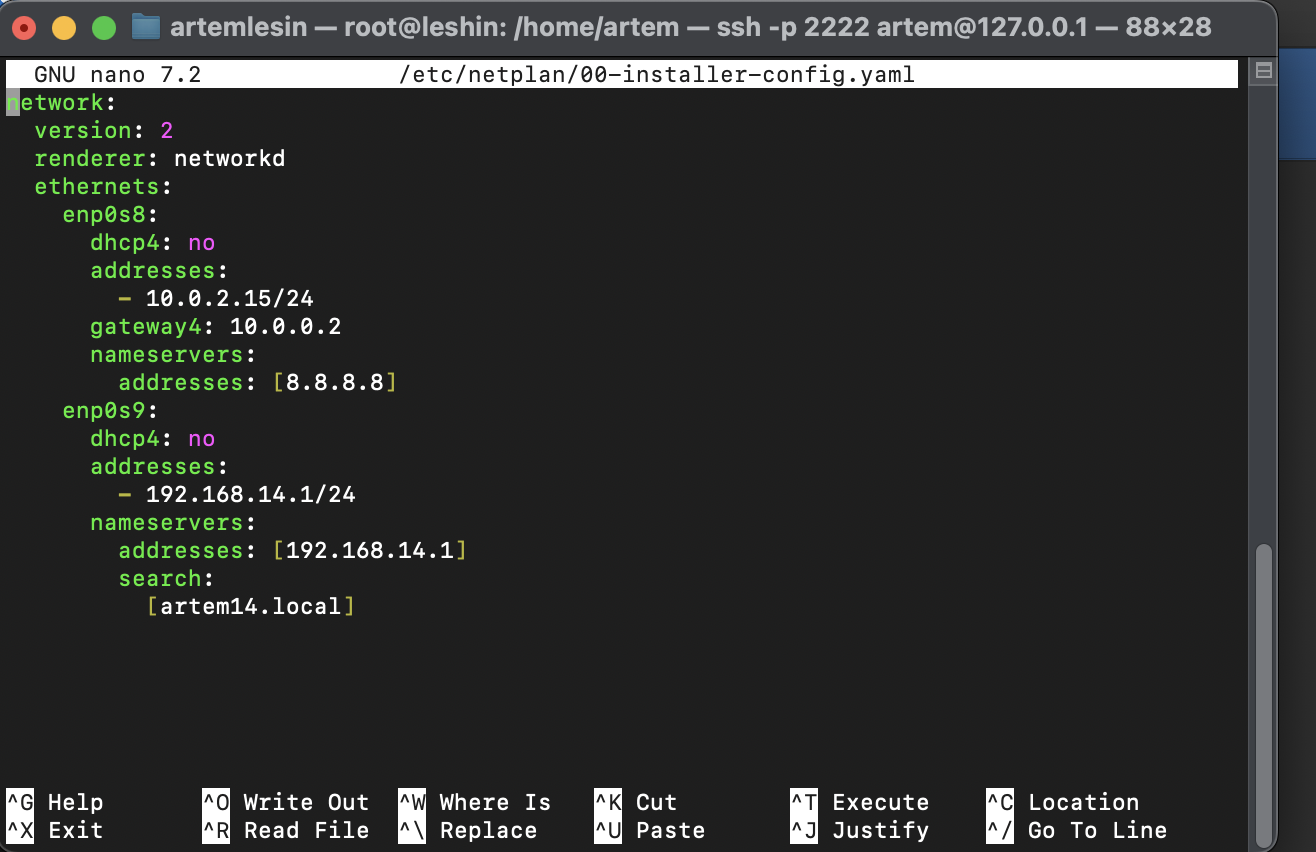
\includegraphics[width=0.8\textwidth]{photo/snimok7.png}
    \caption{Настройки сети в файле 00-installer-config.yaml}
    \label{fig:00-installer-config.yaml}
\end{figure}

После перезагрузки сервера проверяется самоопределение имени хоста. На \hyperref[fig:hostname-check]{рисунке \ref*{fig:hostname-check}} представлен результат проверки.

\begin{figure}[H]
    \centering
    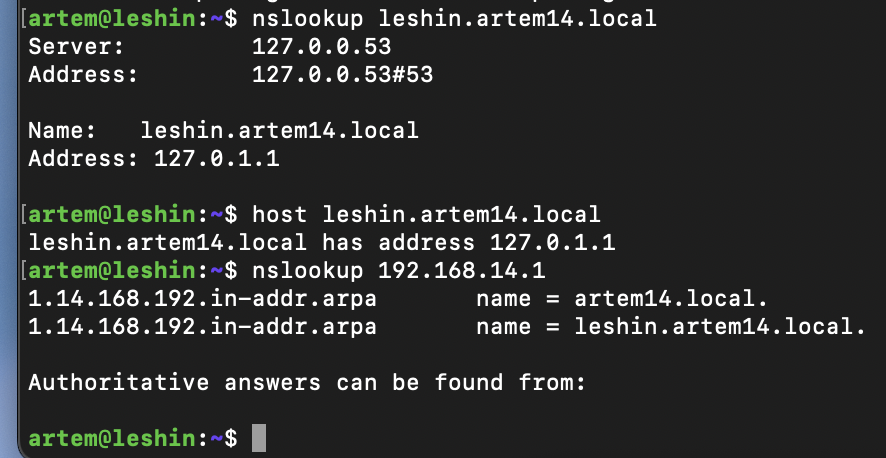
\includegraphics[width=0.6\textwidth]{photo/snimok8.png}
    \caption{Проверка имени хоста}
    \label{fig:hostname-check}
\end{figure}

\section{Настройка динамического обновления DNS зон}

Для обеспечения динамического обновления DNS-записей необходимо настроить совместную работу DHCP-сервера с DNS. На \hyperref[fig:dhcpd.conf]{рисунке \ref*{fig:dhcpd.conf}} представлена конфигурация файла \texttt{dhcpd.conf}, в которой добавлены параметры для обновления DNS-зон.

\begin{figure}[H]
    \centering
    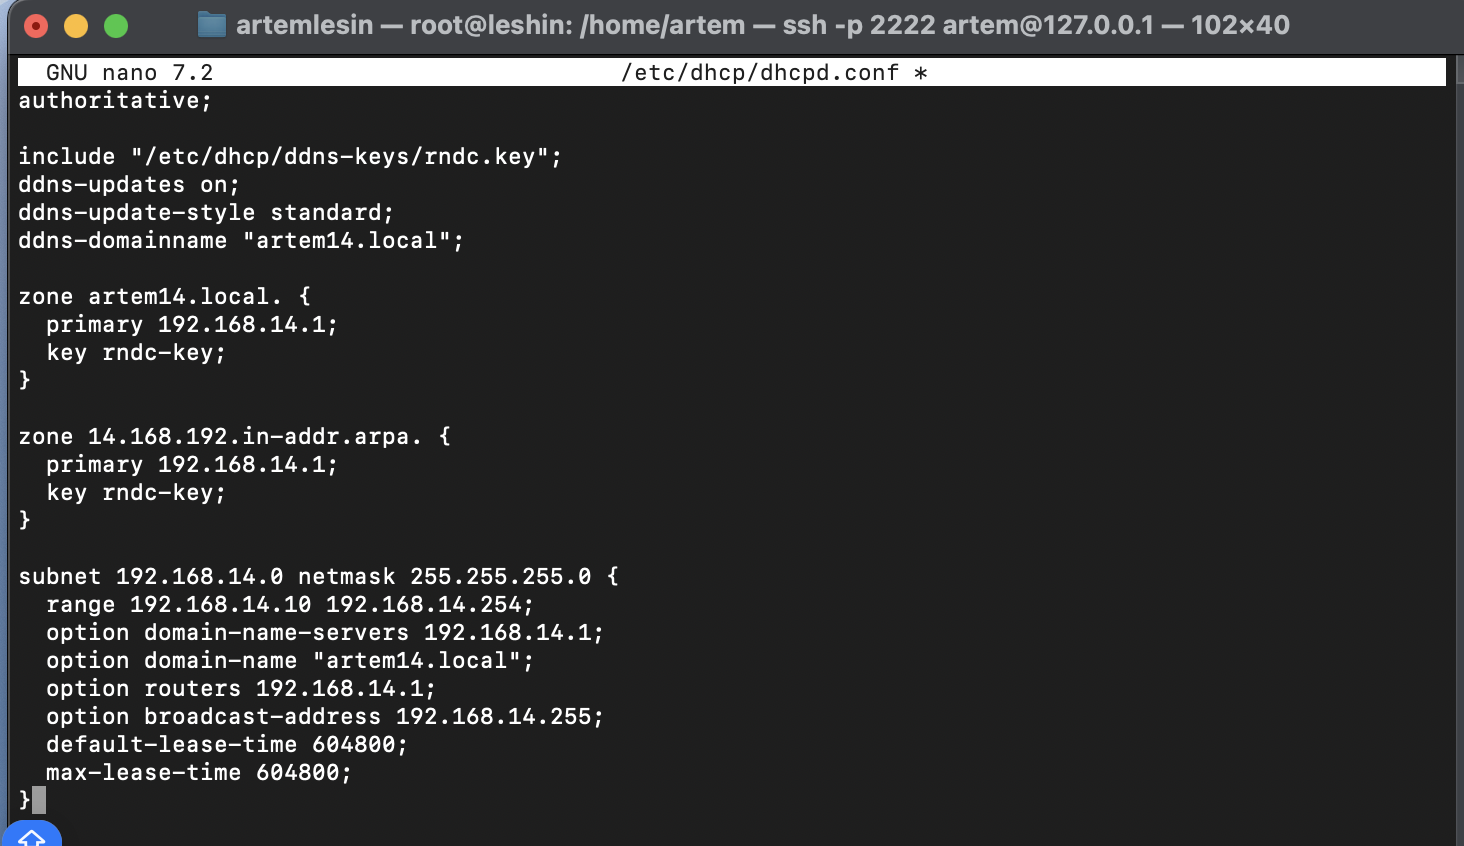
\includegraphics[width=0.8\textwidth]{photo/snimok9.png}
    \caption{Конфигурация DHCP-сервера}
    \label{fig:dhcpd.conf}
\end{figure}

\section{Проверка работоспособности}

После выполнения всех настроек выполняется проверка работы DNS-сервера. На \hyperref[fig:dns-check]{рисунке \ref*{fig:dns-check}} представлен результат выполнения запроса по имени, демонстрирующий успешное возвращение IP-адреса.

\begin{figure}[H]
    \centering
    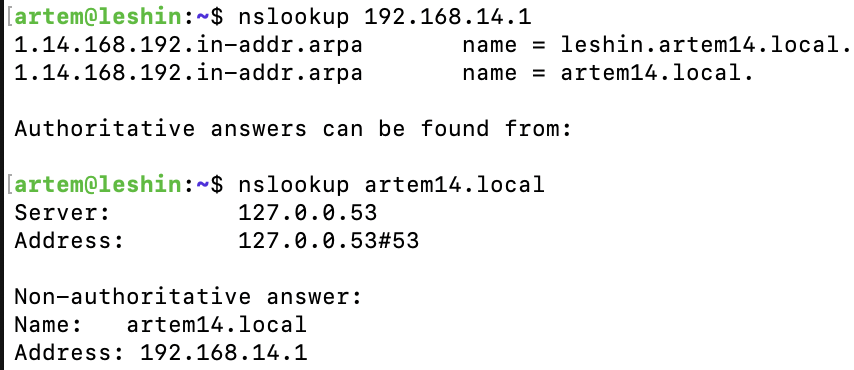
\includegraphics[width=0.8\textwidth]{photo/snimok10.png}
    \caption{Проверка работы DNS-сервера}
    \label{fig:dns-check}
\end{figure}

\section*{Заключение}
\addcontentsline{toc}{section}{Заключение}

В ходе выполнения работы был настроен DNS-сервер на базе Bind9, а также организована его совместная работа с DHCP-сервером с возможностью динамического обновления DNS-зон. Выполнены следующие задачи:
\begin{enumerate}
    \item изменено имя хоста сервера;
    \item установлен и настроен DNS-сервер Bind9;
    \item созданы зоны прямого и обратного просмотра;
    \item настроено динамическое обновление DNS-зон DHCP-сервером;
    \item выполнена проверка работоспособности всех компонентов.
\end{enumerate}

\end{document}